\documentclass[
	a4paper,
	oneside,
	BCOR = 10mm,
	DIV = 12,
	12pt,
	headings = normal,
]{scrartcl}

%%% Length calculations
\usepackage{calc}
%%%

%%% Support for color
\usepackage{xcolor}
\definecolor{lightblue}{HTML}{03A9F4}
\definecolor{red}{HTML}{F44336}
%%%

%%% Including graphics
\usepackage{graphicx}
%%%

%%% Font selection
\usepackage{fontspec}

\setromanfont{STIX Two Text}[
	SmallCapsFeatures = {LetterSpace = 8},
]

\setsansfont{IBM Plex Sans}[
	Scale = MatchUppercase,
]

\setmonofont{IBM Plex Mono}[
	Scale = MatchUppercase,
]
%%%

%%% Math typesetting
\usepackage{amsmath}

\usepackage{unicode-math}
\setmathfont{STIX Two Math}

\usepackage{IEEEtrantools}
%%%

%%% List settings
\usepackage{enumitem}
\setlist[enumerate]{
	label*      = {\arabic*.},
	left        = \parindent,
	topsep      = 0\baselineskip,
	parsep      = 0\baselineskip,
	noitemsep, % override itemsep
}
% List settings for levels 2–4
\setlist[enumerate, 2, 3, 4]{
	label*      = {\arabic*.},
	left        = 0em,
	topsep      = 0\baselineskip,
	parsep      = 0\baselineskip,
	noitemsep, % override itemsep
}

\setlist[itemize]{
	label*      = {—},
	left        = \parindent,
	topsep      = 0\baselineskip,
	parsep      = 0\baselineskip,
	itemsep     = 1\baselineskip,
	noitemsep, % override itemsep
}

\setlist[description]{
	font        = {\rmfamily\upshape\bfseries},
	topsep      = 1\baselineskip,
	parsep      = 0\baselineskip,
	itemsep     = 0\baselineskip,
}

%%%

%%% Structural elements typesetting
\setkomafont{pagenumber}{\rmfamily\upshape}
\setkomafont{disposition}{\rmfamily\bfseries}

% Sectioning
\RedeclareSectionCommand[
	beforeskip = -1\baselineskip,
	afterskip  = 1\baselineskip,
	font       = {\normalsize\bfseries\scshape},
]{section}

\RedeclareSectionCommand[
	beforeskip = -1\baselineskip,
	afterskip  = 1\baselineskip,
	font       = {\normalsize\bfseries\itshape},
]{subsection}

\RedeclareSectionCommand[
	beforeskip = -1\baselineskip,
	afterskip  = 1\baselineskip,
	font       = {\normalsize\bfseries},
]{subsubsection}

\RedeclareSectionCommand[
	beforeskip = -1\baselineskip,
	afterskip  = -0.5em,
	font       = {\normalsize\mdseries\scshape\addfontfeatures{Letters = {UppercaseSmallCaps}}},
]{paragraph}
%%%

%%% Typographic enhancements
\usepackage{microtype}
%%%

%%% Language-specific settings
\usepackage{polyglossia}
\setmainlanguage{ukrainian}
\setotherlanguages{english}
%%%

%%% Captions
\usepackage{caption}
\usepackage{subcaption}

%\DeclareCaptionLabelFormat{closing}{#2)}
%\captionsetup[subtable]{labelformat = closing}

%\captionsetup[subfigure]{labelformat = closing}

\captionsetup[table]{
	aboveskip = 0\baselineskip,
	belowskip = 0\baselineskip,
}

\captionsetup[figure]{
	aboveskip = 1\baselineskip,
	belowskip = 0\baselineskip,
}

\captionsetup[subfigure]{
	labelformat = simple,
	labelformat = brace,
}
%%%

%%% Hyphenated ragged typesetting
\usepackage{ragged2e}
%%%

%%% Table typesetting
\usepackage{booktabs}
\usepackage{longtable}

\usepackage{multirow}

\usepackage{array}
\newcolumntype{v}[1]{>{\RaggedRight\arraybackslash\hspace{0pt}}p{#1}}
\newcolumntype{b}[1]{>{\Centering\arraybackslash\hspace{0pt}}p{#1}}
\newcolumntype{n}[1]{>{\RaggedLeft\arraybackslash\hspace{0pt}}p{#1}}
%%%

%%% Drawing
\usepackage{tikz}
\usepackage{tikzscale}
\usetikzlibrary{positioning}
\usetikzlibrary{arrows.meta} % Stealth arrow tips
%%%

%%% SI units typesetting
\usepackage{siunitx}
\sisetup{
	output-decimal-marker = {,},
	exponent-product      = {\cdot},
	inter-unit-product    = \ensuremath{{} \cdot {}},
	per-mode              = symbol,
}
%%%

% Code Highlighting
\usepackage{minted}
\setmintedinline{
	style = bw,
	breaklines,
}

\newminted[bashterm]{bash}{%
	autogobble,%
	style=bw,%
}

\newminted[codegeneric]{text}{%
	autogobble,%
	style=bw,%
	breaklines,%
	fontsize=\small,%
}

\newmintinline{bash}{%
}

\newmintinline[minttext]{text}{%
	breaklines,%
}

%%% Framing code listings
\usepackage{tcolorbox}
\tcbuselibrary{breakable}
\tcbuselibrary{minted}
\tcbuselibrary{skins}

% Text file listing
\newtcblisting[
	auto counter,
	list inside,
	number within = section,
]{listingplaintext}[3][]{%
	minted language = text,
	minted style    = bw,
	minted options  = {
		autogobble,
		linenos,
		tabsize = 4,
		breaklines,
		breakanywhere,
		fontsize = \footnotesize,
	},
	empty,
	sharp corners,
	coltitle = black,
	borderline horizontal = {1pt}{0pt}{black},
	titlerule = {0.5pt},
	titlerule style = {
		black,
	},
	toptitle = 0.3em,
	bottomtitle = 0.3em,
	before skip      = \intextsep,
	after  skip      = \intextsep,
	title            = {Лістинг \thetcbcounter: #2},
	list entry       = {\protect\numberline{\thetcbcounter}#2},
	left = 0em,
	right = 0em,
	%
	listing only,
	breakable,
	%
	label = {#3},%
}

\newtcblisting[
	use counter from = listingplaintext,
	list inside,
	number within = section,
]{listingpython}[3][]{%
	minted language = python,
	minted style    = bw,
	minted options  = {
		autogobble,
		linenos,
		tabsize = 4,
		breaklines,
		breakanywhere,
		fontsize = \footnotesize,
	},
	empty,
	sharp corners,
	coltitle = black,
	borderline horizontal = {1pt}{0pt}{black},
	titlerule = {0.5pt},
	titlerule style = {
		black,
	},
	toptitle = 0.3em,
	bottomtitle = 0.3em,
	before skip      = \intextsep,
	after  skip      = \intextsep,
	title            = {Лістинг \thetcbcounter: #2},
	list entry       = {\protect\numberline{\thetcbcounter}#2},
	left = 0em,
	right = 0em,
	%
	listing only,
	breakable,
	%
	label = {#3},
	%
	#1%
}

\newtcbinputlisting[
	use counter from = listingplaintext,
	list inside,
	number within = section
]{\inputpython}[4][]{%
	minted language = python,
	minted style    = bw,
	minted options  = {
		autogobble,
		linenos,
		tabsize = 4,
		breaklines,
		breakanywhere,
		fontsize = \footnotesize,
	},
	empty,
	sharp corners,
	coltitle = black,
	borderline horizontal = {1pt}{0pt}{black},
	titlerule = {0.5pt},
	titlerule style = {
		black,
	},
	toptitle = 0.3em,
	bottomtitle = 0.3em,
	before skip      = \intextsep,
	after  skip      = \intextsep,
	title            = {Лістинг \thetcbcounter: #3},
	list entry       = {\protect\numberline{\thetcbcounter}#3},
	left = 0em,
	right = 0em,
	%
	listing file={#2},
	listing only,
	breakable,
	%
	label = {#4}
}

% Linux command-line listing
\newtcblisting{linuxterm}%
{%
	% Syntax highlighing options
	listing only,%
	minted language = bash,%
	minted options={%
		autogobble,%
		linenos%
	},%
	% Presentation options
	empty,%
	%% Margins
	sharp corners,%
	toptitle = 0.0em,%
	bottomtitle = 0.0em,%
	left = 0em,%
	right = 0em,%
	before skip = \intextsep,%
	after skip = \intextsep,%
}

\newtcblisting{linuxtermout}%
{%
	% Syntax highlighing options
	listing only,%
	minted language = text,%
	minted options={%
		autogobble,%
		linenos%
	},%
	% Presentation options
	empty,%
	%% Margins
	sharp corners,%
	toptitle = 0.0em,%
	bottomtitle = 0.0em,%
	left = 0em,%
	right = 0em,%
	before skip = \intextsep,%
	after skip = \intextsep,%
}

% Dockerfile listings
\newtcblisting[
	use counter from = listingplaintext,
	list inside,
	number within = section,
]{listingdocker}[3][]{%
	minted language = dockerfile,
	minted style    = bw,
	minted options  = {
		autogobble,%
		linenos,
		tabsize = 4,
		breaklines,
		breakanywhere,
		fontsize = \footnotesize,
	},
	empty,
	sharp corners,
	coltitle = black,
	borderline horizontal = {1pt}{0pt}{black},
	titlerule = {0.5pt},
	titlerule style = {
		black,
	},
	toptitle = 0.3em,
	bottomtitle = 0.3em,
	before skip      = \intextsep,
	after  skip      = \intextsep,
	title            = {Лістинг \thetcbcounter: #2},
	list entry       = {\protect\numberline{\thetcbcounter}#2},
	left = 0em,
	right = 0em,
	%
	listing only,
	breakable,
	%
	label = {#3},%
}

% Docker Compose listings
\newtcblisting[
	use counter from = listingplaintext,
	list inside,
	number within = section,
]{listingdockercompose}[3][]{%
	minted language = yaml,
	minted style    = bw,
	minted options  = {
		autogobble,%
		linenos,
		tabsize = 4,
		breaklines,
		breakanywhere,
		fontsize = \footnotesize,
	},
	empty,
	sharp corners,
	coltitle = black,
	borderline horizontal = {1pt}{0pt}{black},
	titlerule = {0.5pt},
	titlerule style = {
		black,
	},
	toptitle = 0.3em,
	bottomtitle = 0.3em,
	before skip      = \intextsep,
	after  skip      = \intextsep,
	title            = {Лістинг \thetcbcounter: #2},
	list entry       = {\protect\numberline{\thetcbcounter}#2},
	left = 0em,
	right = 0em,
	%
	listing only,
	breakable,
	%
	label = {#3},%
}


% Customize minted line numbers
\renewcommand{\theFancyVerbLine}{\ttfamily\scriptsize\arabic{FancyVerbLine}}

%%%

%%% Typeset menus and keys
\usepackage{menukeys}[
	os=win,
]
%%%

%%% Including full PDF documents
\usepackage{pdfpages}
%%%

%%% Links and hyperreferences
\usepackage{hyperref}
\hypersetup{
	bookmarksnumbered = true,
	colorlinks      = false,
	linkbordercolor = red,
	urlbordercolor  = lightblue,
	pdfborderstyle  = {/S/U/W 1.5},
}
%%%

%%% Length adjustment

% Set baselineskip, default is 14.5 pt
\linespread{1.068966} % ~15.5 pt
\setlength{\emergencystretch}{1em}
\setlength{\parindent}{1.5em}
\newlength{\gridunitwidth}
\setlength{\gridunitwidth}{\textwidth / 12}
%%%

%%% Custom commands
\newcommand{\allcaps}[1]{%
	{%
		\addfontfeatures{%
			Letters = UppercaseSmallCaps,
			LetterSpace = 8,%
		}%
		#1%
	}%
}
\newcommand{\filename}[1]{\texttt{#1}}
\newcommand{\progname}[1]{\texttt{#1}}
\newcommand{\commandname}[1]{\texttt{#1}}
\newcommand{\modulename}[1]{\texttt{#1}}
\newcommand{\transeng}[1]{{англ.}~\textit{\textenglish{#1}}}
%%%

%%% Custom math commands
\newcommand{\longvar}[1]{\mathit{#1}}
%%%

\begin{document}

\begin{titlepage}
		\begin{center}
			Міністерство освіти і~науки України\\
			Національний авіаційний університет\\
			Факультет кібербезпеки, комп'ютерної та програмної інженерії\\
			Кафедра комп'ютеризованих систем управління

			\vspace{\fill}
				Лабораторна робота №~1.1\\
				з~дисципліни «Технології проектування комп'ютерних систем»\\
				на~тему «Зображення графічних об'єктів в програмі~\textenglish{Auto\allcaps{CAD}}»\\
				Варіант №~8

			\vspace{\fill}

			\begin{flushright}
				Виконав:\\
				студент \allcaps{ФККПІ}\\
				групи \allcaps{СП}-425\\
				Клокун В.\,Д.\\
				Перевірила:\\
				Голего Н.\,М.
			\end{flushright}

			Київ 2019
		\end{center}
	\end{titlepage}

	\tableofcontents
	\clearpage

	\section{Мета роботи}
		Ознайомлення з~пакетом проектування~\textenglish{Auto\allcaps{CAD}}. Оволодіння основними прийомами зображення простих графічних об'єктів в~програмі~\textenglish{Auto\allcaps{CAD}}.

	\section{Хід~роботи}
		\subsection{Рисування зовнішньої і~внутрішньої рамок формату~\textenglish{A4}}
			Рисуємо зовнішню і~внутрішню рамки формату~\textenglish{A4}. Для~цього вводимо і~виконуємо такі команди:
			\begin{codegeneric}
				Command: rectangle
				Specify first corner point or [Chamfer/Elevation/Fillet/Thickness/Width]: 0,0
				Specify other corner point or [Area/Dimensions/Rotation]: 210,297
			\end{codegeneric}
			Тепер зовнішня рамка нарисована~(рис.~\ref{subfig:01-borders-01}). Рисуємо внутрішню рамку. Для~цього виконуємо такі команди:
			\begin{codegeneric}
				Command: rectangle
				Specify first corner point or [Chamfer/Elevation/Fillet/Thickness/Width]: 20,5
				Specify other corner point or [Area/Dimensions/Rotation]: @185,287
			\end{codegeneric}

			\begin{figure}[!htbp]
				\begin{subfigure}[b]{0.5\columnwidth}
					\centering
					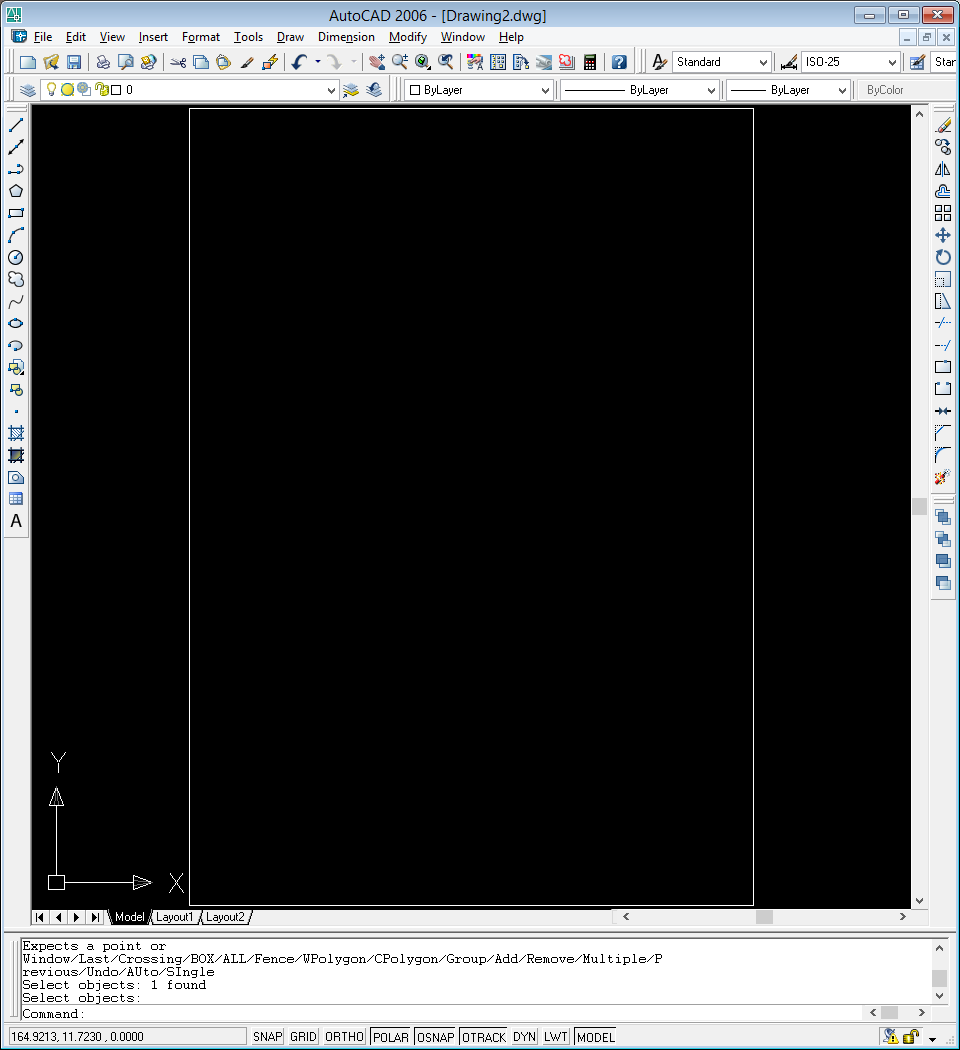
\includegraphics[height=13\baselineskip]{./assets/y04s01-csdt-lab-01-01-p01.png}
					\caption{}
					\label{subfig:01-borders-01}
				\end{subfigure}%
				\begin{subfigure}[b]{0.5\columnwidth}
					\centering
					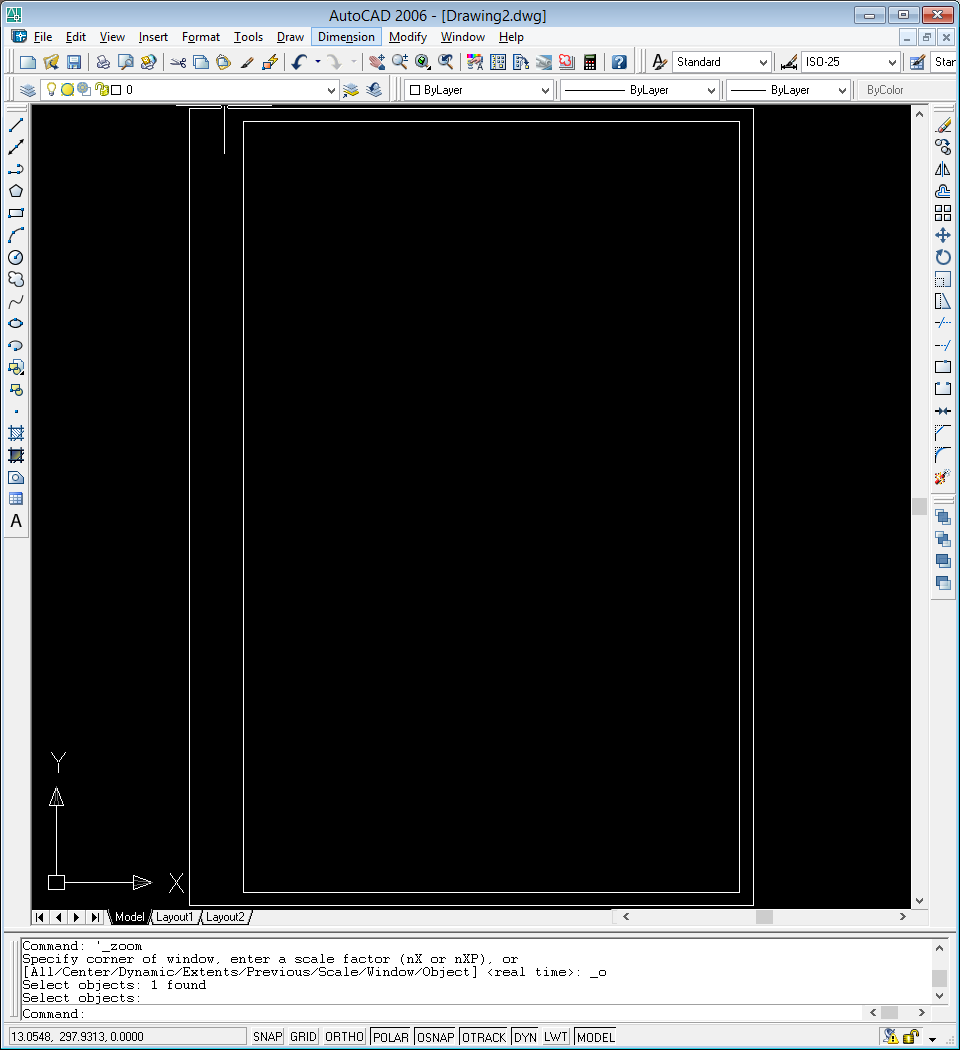
\includegraphics[height=13\baselineskip]{./assets/y04s01-csdt-lab-01-01-p02.png}
					\caption{}
					\label{subfig:01-borders-02}
				\end{subfigure}%
				\caption{Результат рисування рамок: \subref{subfig:01-borders-01}~— зовнішньої, \subref{subfig:01-borders-02}~— внутрішньої}
				\label{fig:01-borders}
			\end{figure}

		\subsection{Рисування відрізків прямих}
			Для~виконання завдання необхідно нарисувати такі відрізки прямих:
			\begin{enumerate}
				\item Горизонтальний відрізок прямої завдовжки \SI{50}{\milli\metre}, виконаний суцільною лінією.
				\item Горизонтальний відрізок прямої завдовжки \SI{50}{\milli\metre}, виконаний штриховою лінією.
				\item Горизонтальний відрізок прямої завдовжки \SI{50}{\milli\metre}, виконаний штрих-пунктирною лінією.
				\item Відрізок похилої прямої завдовжки \SI{50}{\milli\metre} під~кутом \SI{25}{\degree}, виконаний тонкою суцільною лінією.
			\end{enumerate}

			Щоб~нарисувати ці~відрізки, необхідно завантажити штрихову і~штрих-пунктирну лінії. Спочатку додамо штрихову лінію. Для~цього заходимо в~меню \menu{Format > Linetype...}~— відкриється вікно~«Менеджер типів ліній»~(\transeng{Linetype Manager}, рис.~\ref{subfig:02-linetypes-01}). У~відкрившомуся Менеджері натискаємо кнопку «\textenglish{Load}»~— відкриється вікно~«Завантажити або~перезавантажити типи ліній»~(\transeng{Load or Reload Linetypes}, рис.~\ref{subfig:02-linetypes-02}). У~з'явившомуся вікні вибираємо тип~лінії \textenglish{ACAD\_ISO02W100 (\allcaps{ISO} dash)} і~натискаємо кнопку~«\textenglish{\allcaps{OK}}»~— ми~додали штриховий тип~лінії. Тепер повторюємо вищеописані дії~для~штрих-пунктирної лінії (\textenglish{ACAD\_ISO08W100 (\allcaps{ISO} long-dash short-dash)}).

			\begin{figure}[!htbp]
				\begin{subfigure}[b]{0.5\columnwidth}
					\centering
					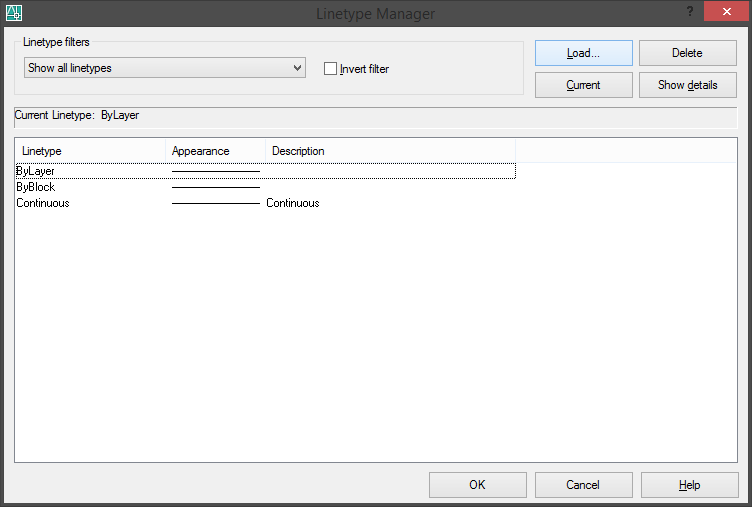
\includegraphics[height=9\baselineskip]{./assets/y04s01-csdt-lab-01-01-p03.png}
					\caption{}
					\label{subfig:02-linetypes-01}
				\end{subfigure}%
				\begin{subfigure}[b]{0.5\columnwidth}
					\centering
					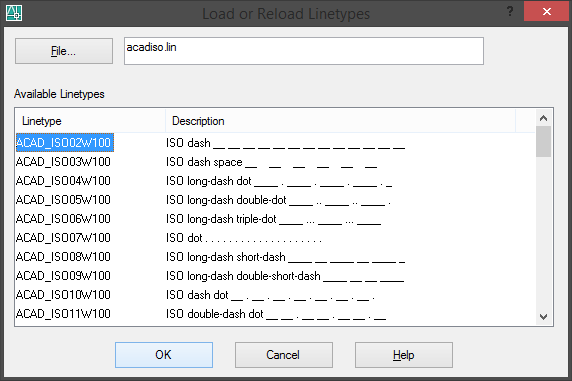
\includegraphics[height=9\baselineskip]{./assets/y04s01-csdt-lab-01-01-p04.png}
					\caption{}
					\label{subfig:02-linetypes-02}
				\end{subfigure}%
				\caption{Вікна завантаження типів ліній: \subref{subfig:02-linetypes-01}~— Менеджер типів ліній, \subref{subfig:02-linetypes-02}~— Завантажити або~перезавантажити типи ліній}
				\label{fig:02-linetypes}
			\end{figure}

			Рисуємо 3~горизонтальні відрізки за~допомогою таких команд:
			\begin{codegeneric}
				Command: line
				Specify first point: 25,280
				Specify next point or [Undo]: 75,280
				Specify next point or [Undo]: *Cancel*
				Command: line
				Specify first point: 25,270
				Specify next point or [Undo]: @50,0
				Specify next point or [Undo]: *Cancel*
				Command: line
				Specify first point: 25,260
				Specify next point or [Undo]: @50,0
				Specify next point or [Undo]: *Cancel*
			\end{codegeneric}
			Нарисувавши ці~відрізки, задаємо тип~їх~ліній. Для~цього покроково обираємо кожен відрізок, натиснувши на~нього курсором, та~обираємо тип~його лінії у~відповідному меню.

			Тепер рисуємо похилий відрізок. Для~цього виконуємо таку команду:
			\begin{codegeneric}
				Command: line
				Specify first point: 25,230
				Specify next point or [Undo]: @55<25
				Specify next point or [Undo]: *Cancel*
			\end{codegeneric}
			Після того, як~ми~нарисували похилий відрізок, встановлюємо для~нього штрих-пунктирний тип~лінії. В результаті ми побудували необхідні відрізки~(рис.~\ref{fig:03-lines}).

			\begin{figure}[!htbp]
				\centering
				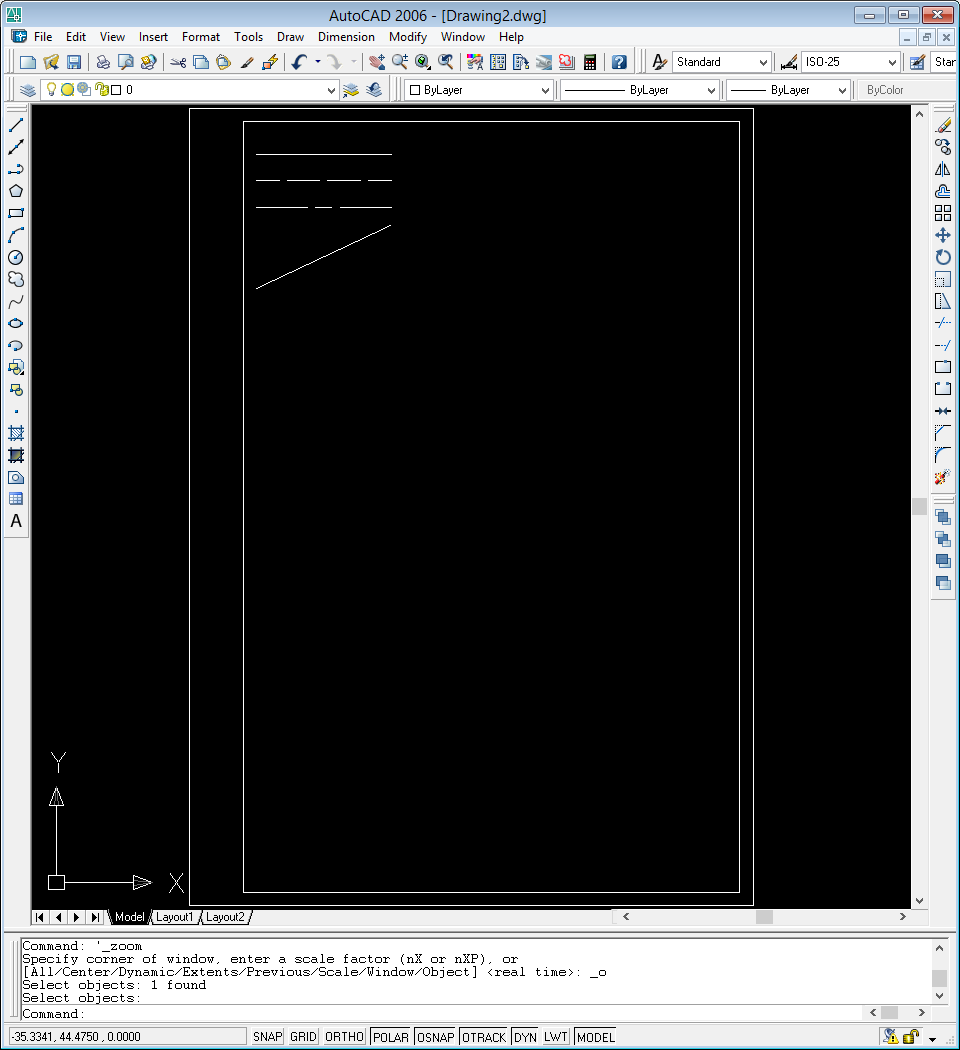
\includegraphics[height=18\baselineskip]{./assets/y04s01-csdt-lab-01-01-p05.png}
				\caption{Документ після рисування відрізків}
				\label{fig:03-lines}
			\end{figure}

		\subsection{Побудова правильних многокутників за~описаним навколо них~колом}
			Щоб~побудувати правильні многокутники за~описаним навколо них~колом, спочатку ввімкнемо прив'язку до~об'єктів~(\transeng{Object snapping}). Для~цього наводимо курсор на~кнопку~«\textenglish{\allcaps{OSNAP}}», натискаємо на~неї~правою клавішею миші і~вмикаємо прив'язку. Також вмикаємо прив'язку до~кінцевої точки~(\transeng{endpoint}), центра~(\transeng{center}) і~перетину~(\transeng{intersection}).

			Тепер будуємо осьові лінії для~многокутника. Для~цього виконуємо такі команди:
			\begin{codegeneric}
				Command: line
				Specify first point: 25,230
				Specify next point or [Undo]: @55<25
				Specify next point or [Undo]: *Cancel*
				Specify first point: 115,285
				Specify next point or [Undo]: @70<-90
				Specify next point or [Undo]: *Cancel*
			\end{codegeneric}
			Змінюємо тип~осьових ліній на~штрих-пунктирні і~переходимо до~побудови многокутників.

			Щоб~побудувати вписаний 6-кутник діаметром~\SI{60}{\milli\metre}, необхідно виконати такі команди:
			\begin{codegeneric}
				Command: polygon
				Enter number of sides <6>: 6
				Specify center of polygon or [Edge]: 115,250
				Enter an option [Inscribed in circle/Circumscribed about circle] <I>: I
				Specify radius of circle: 30
			\end{codegeneric}
			Також, щоб~вказати центр бажаного многокутника, замість команди~\minttext{Specify center of polygon or [Edge]: 115,250} можна навести курсор миші на~точку перетину осьових ліній, і~програма сама визначить бажану координату за~допомогою прив'язки об'єктів, яку~ми~ввімкнули раніше.

			Щоб~побудувати 5-кутник діаметром~\SI{50}{\milli\metre}, також побудуємо осьові лінії для~нього. Для~цього використаємо такі команди:
			\begin{codegeneric}
				Command: line
				Specify first point: 140,240
				Specify next point or [Undo]: @60<0
				Specify next point or [Undo]: *Cancel*
				Command: line
				Specify first point: 170,270
				Specify next point or [Undo]: @60<-90
				Specify next point or [Undo]: *Cancel*
			\end{codegeneric}
			Побудувавши осьові лінії, будуємо бажаний многокутник за~допомогою таких команд:
			\begin{codegeneric}
				Command: polygon
				Enter number of sides <6>: 5
				Specify center of polygon or [Edge]: 170,240
				Enter an option [Inscribed in circle/Circumscribed about circle] <I>: I
				Specify radius of circle: 25
			\end{codegeneric}
			В~результаті побудували бажані многокутники~(рис.~\ref{fig:04-polygons}).

			\begin{figure}[!htbp]
				\centering
				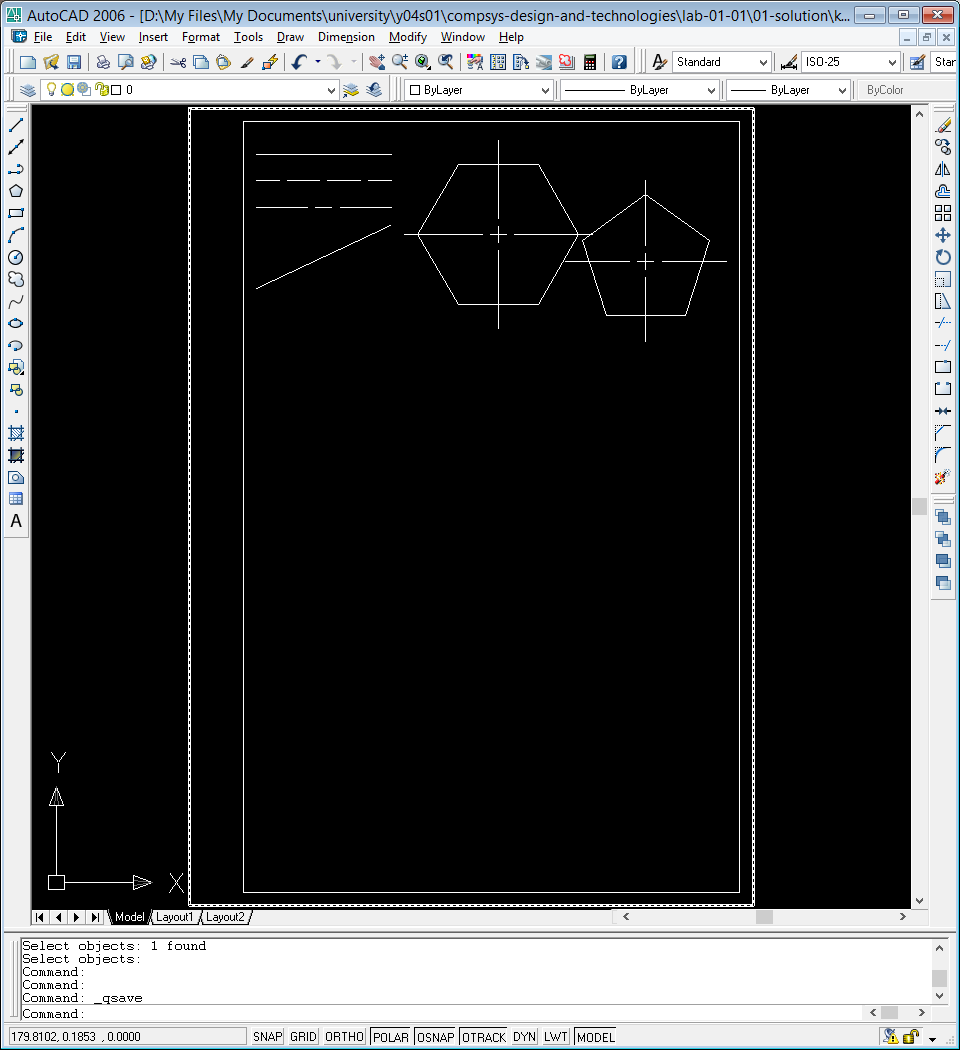
\includegraphics[height=19\baselineskip]{./assets/y04s01-csdt-lab-01-01-p06.png}
				\caption{Вигляд документа після побудови многокутників}
				\label{fig:04-polygons}
			\end{figure}

		\subsection{Побудова еліпса за~великою та~малою осями}
			Щоб~побудувати еліпс, спочатку побудуємо його осьові лінії. Для~цього скопіюємо осьові лінії, які~ми~використовували для~побудови многокутників, за~допомогою таких команд:
			\begin{codegeneric}
				Command: copy
				Select objects: 1 found
				Select objects: 1 found, 2 total
				Select objects:
				Specify base point or [Displacement] <Displacement>: 55,-70
				Specify second point or <use first point as displacement>:
			\end{codegeneric}
			Тут~виділення об'єктів виконується за~допомогою курсора миші. Коли виділені всі~потрібні об'єкти, необхідно натиснути~\keys{\return}.

			Створивши необхідні осьові лінії, будуємо власне еліпс. Для~цього використовуємо такі команди:
			\begin{codegeneric}
				Command: ellipse
				Specify axis endpoint of ellipse or [Arc/Center]: c
				Specify center of ellipse: 170,180
				Specify endpoint of axis: @25,0
				Specify distance to other axis or [Rotation]: @15,0
			\end{codegeneric}
			В~результаті побудували еліпс~(рис.~\ref{fig:05-ellipse}).

			\begin{figure}[!htbp]
				\centering
				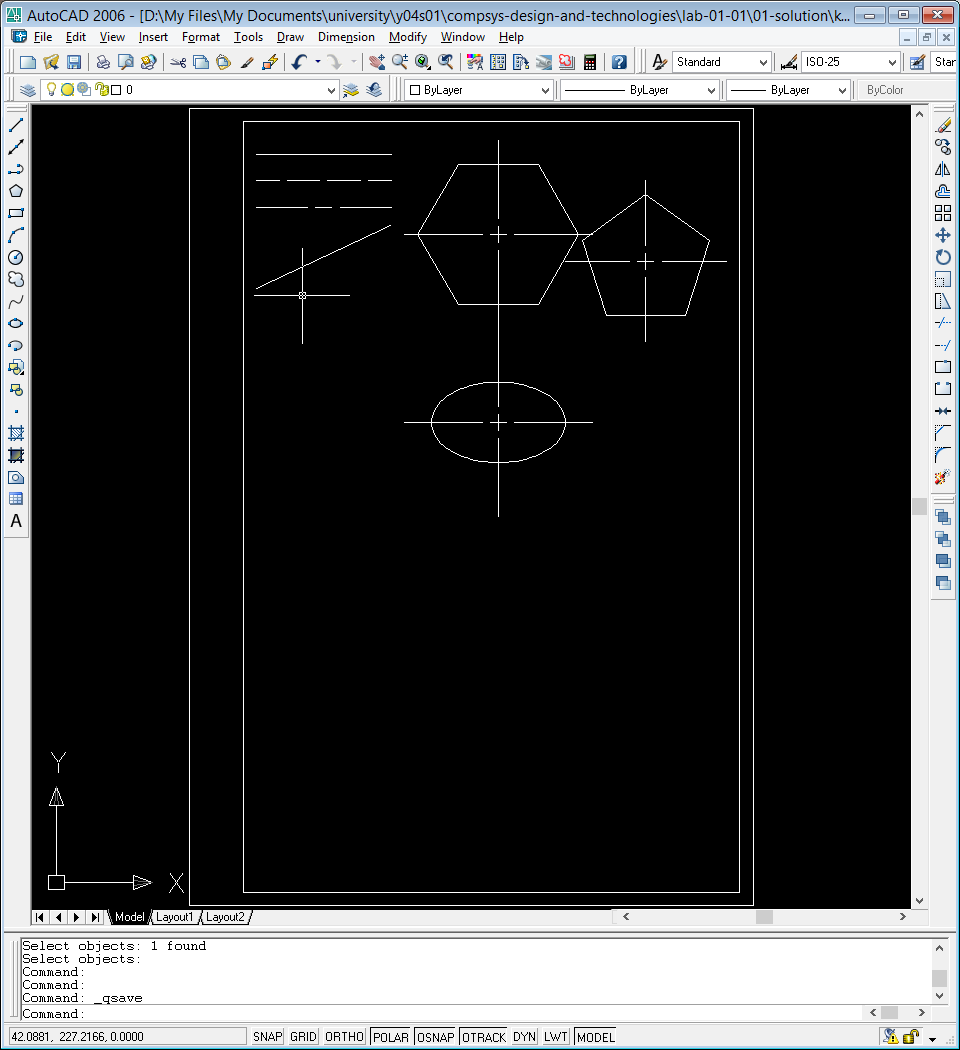
\includegraphics[height=20\baselineskip]{./assets/y04s01-csdt-lab-01-01-p07.png}
				\caption{Вигляд документа після побудови еліпса}
				\label{fig:05-ellipse}
			\end{figure}

		\subsection{Побудова спряження двох кіл}
			Необхідно побудувати два~кола з~радіусами $R_{1} = \SI{15}{\milli\metre}$ і~$R_{2} = \SI{20}{\milli\metre}$ так, щоб~відстань між~їх~центрами~$O_{1}O_{2}$ по~горизонталі дорівнювала \SI{5}{\milli\metre}, а~по~вертикалі~— \SI{45}{\milli\metre}. Також необхідно побудувати спряження цих~кіл, радіус дуги, якою виконують спряження~— \SI{20}{\milli\metre}.

			Щоб~виконати це~завдання, спочатку побудуємо осьові лінії для~першого кола за~допомогою таких команд:
			\begin{codegeneric}
				Command: line
				Specify first point: 100,175
				Specify next point or [Undo]: @40<0
				Specify next point or [Undo]: *Cancel*
				Command: line
				Specify first point: 95,170
				Specify next point or [Undo]: @40<0
				Specify next point or [Undo]: *Cancel*
			\end{codegeneric}
			Тепер копіюємо побудовані осьові лінії для~другого кола за~умовами завдання, виконавши такі команди:
			\begin{codegeneric}
				Command: copy
				2 found
				Specify base point or [Displacement] <Displacement>: 5,-45
				Specify second point or <use first point as displacement>:
			\end{codegeneric}
			Скопіювавши осьові лінії для~обох кіл, будуємо власне кола:
			\begin{codegeneric}
				Command: circle
				Specify center point for circle or [3P/2P/Ttr (tan tan radius)]: 115,170
				Specify radius of circle or [Diameter]: 15
				Command: circle
				Specify center point for circle or [3P/2P/Ttr (tan tan radius)]: 120,125
				Specify radius of circle or [Diameter] <15.0000>: 20
			\end{codegeneric}
			Будуємо спряження кіл:
			\begin{codegeneric}
				Command: fillet
				Current settings: Mode = TRIM, Radius = 0.0000
				Select first object or [Undo/Polyline/Radius/Trim/Multiple]: T
				Enter Trim mode option [Trim/No trim] <Trim>: T
				Select first object or [Undo/Polyline/Radius/Trim/Multiple]: R
				Specify fillet radius <0.0000>: 10
				Select first object or [Undo/Polyline/Radius/Trim/Multiple]:
				Select second object or shift-select to apply corner:
			\end{codegeneric}
			В~результаті ми~побудували два~кола радіусами \SI{15}{\milli\metre} і~\SI{20}{\milli\metre} відповідно, центри яких знаходяться на~горизонтальній відстані у~\SI{5}{\milli\metre} і~вертикальній відстані~\SI{45}{\milli\metre}, спряжені дугою радіусом~\SI{10}{\milli\metre}~(рис.~\ref{fig:06-fillet-circles}).

			\begin{figure}[!htbp]
				\centering
				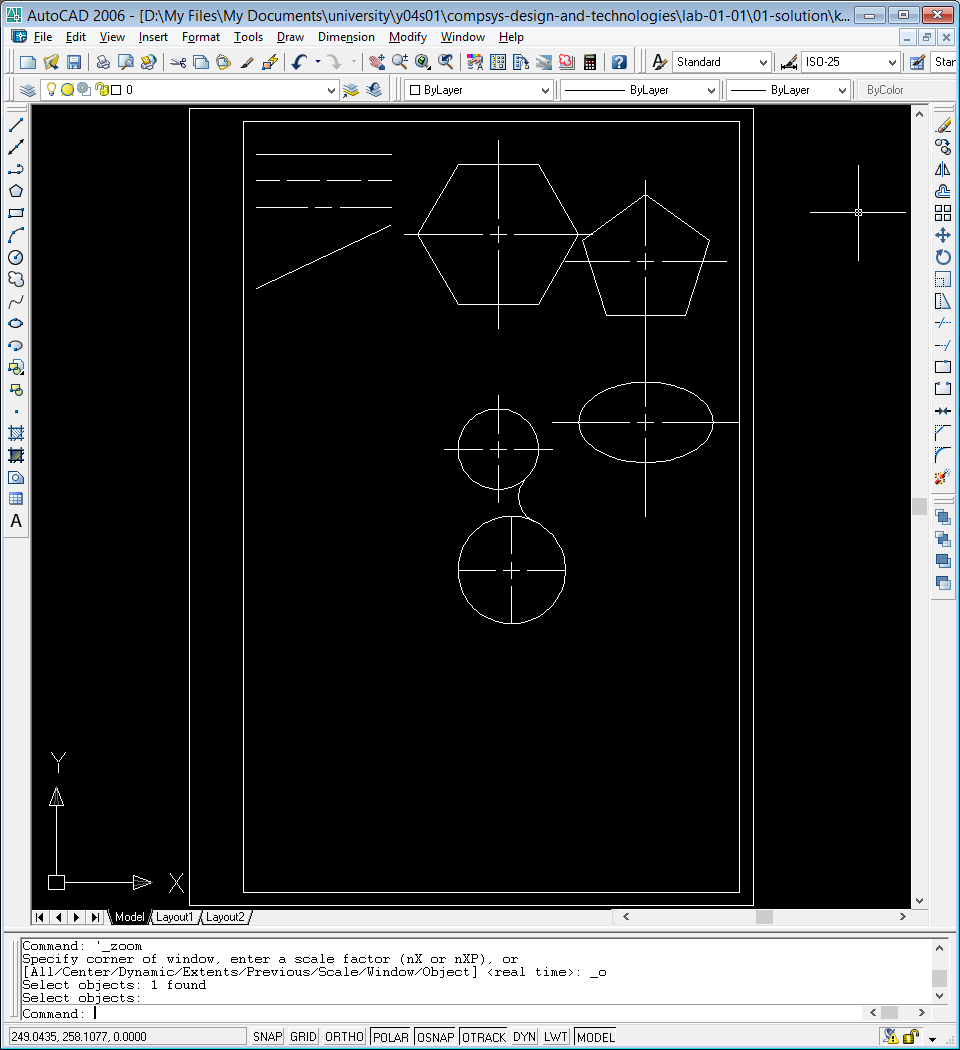
\includegraphics[height=18\baselineskip]{./assets/y04s01-csdt-lab-01-01-p08.png}
				\caption{Вигляд документа після побудови спряжених кіл}
				\label{fig:06-fillet-circles}
			\end{figure}

		\subsection{Побудова спряження двох прямих, що~перетинаються під~кутом~\SI{30}{\degree}}
			Щоб~побудувати спряження прямих, спочатку побудуємо власне прямі. Для~цього виконаємо такі команди:
			\begin{codegeneric}
				Command: line
				Specify first point: 75,225
				Specify next point or [Undo]: @45<210
				Specify next point or [Undo]: *Cancel*
				Command: line
				Specify first point: 25,200
				Specify next point or [Undo]: @60<0
				Specify next point or [Undo]: *Cancel*
			\end{codegeneric}
			Після того, як~прямі побудовані, будуємо їх~спряження:
			\begin{codegeneric}
				Command: fillet
				Current settings: Mode = TRIM, Radius = 10.0000
				Select first object or [Undo/Polyline/Radius/Trim/Multiple]:
				Select second object or shift-select to apply corner:
			\end{codegeneric}
			В~результаті ми~побудували спряження двух прямих: горизонтальної і~нахиленої під~кутом~\SI{30}{\degree}~(рис.~\ref{fig:07-fillet-lines}).

			\begin{figure}[!htbp]
				\centering
				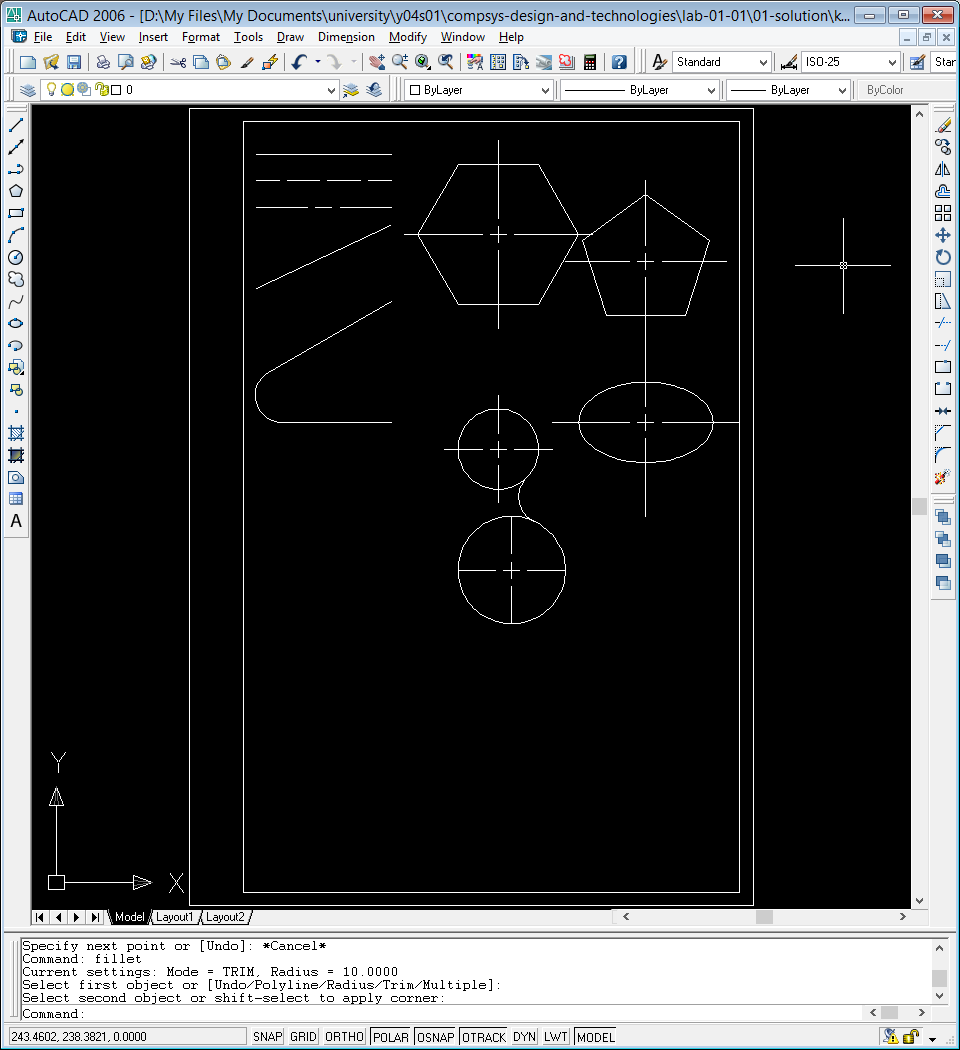
\includegraphics[height=20\baselineskip]{./assets/y04s01-csdt-lab-01-01-p09.png}
				\caption{Вигляд документа після побудови спряжених прямих}
				\label{fig:07-fillet-lines}
			\end{figure}

		\subsection{Побудова фаски висотою~\SI{12}{\milli\metre} під~кутом~\SI{30}{\degree}}
			Щоб~побудувати фаску, спочатку необхідно побудувати прямі, до~яких ми~її~застосуємо. Для~цього використаємо такі команди:
			\begin{codegeneric}
				Command: line
				Specify first point: 75,170
				Specify next point or [Undo]: @-50<0
				Specify next point or [Undo]: *Cancel*
				Command: line
				Specify first point: 25,170
				Specify next point or [Undo]: @50<-90
				Specify next point or [Undo]: *Cancel*
			\end{codegeneric}
			Побудувавши прямі, переходимо до~побудови фаски. За~умовами завдання фаска має~довжину~\SI{12}{\milli\metre} і~виконується під~кутом~\SI{30}{\degree} відносно першої вибраної прямої. Отже, виконуємо такі команди:
			\begin{codegeneric}
				Command: chamfer
				(TRIM mode) Current chamfer Dist1 = 0.0000, Dist2 = 0.0000
				Select first line or [Undo/Polyline/Distance/Angle/Trim/mEthod/Multiple]: A
				Specify chamfer length on the first line <0.0000>: 12
				Specify chamfer angle from the first line <0>: 30
				Select first line or [Undo/Polyline/Distance/Angle/Trim/mEthod/Multiple]:
				Command: chamfer
				(TRIM mode) Current chamfer Length = 12.0000, Angle = 30
				Select first line or [Undo/Polyline/Distance/Angle/Trim/mEthod/Multiple]:
				Select second line or shift-select to apply corner:
			\end{codegeneric}
			В~результаті ми~отримали дві~прямі, з'єднані фаскою із~заданими параметрами~(рис.~\ref{fig:08-chamfer-lines}).

			\begin{figure}[!htbp]
				\centering
				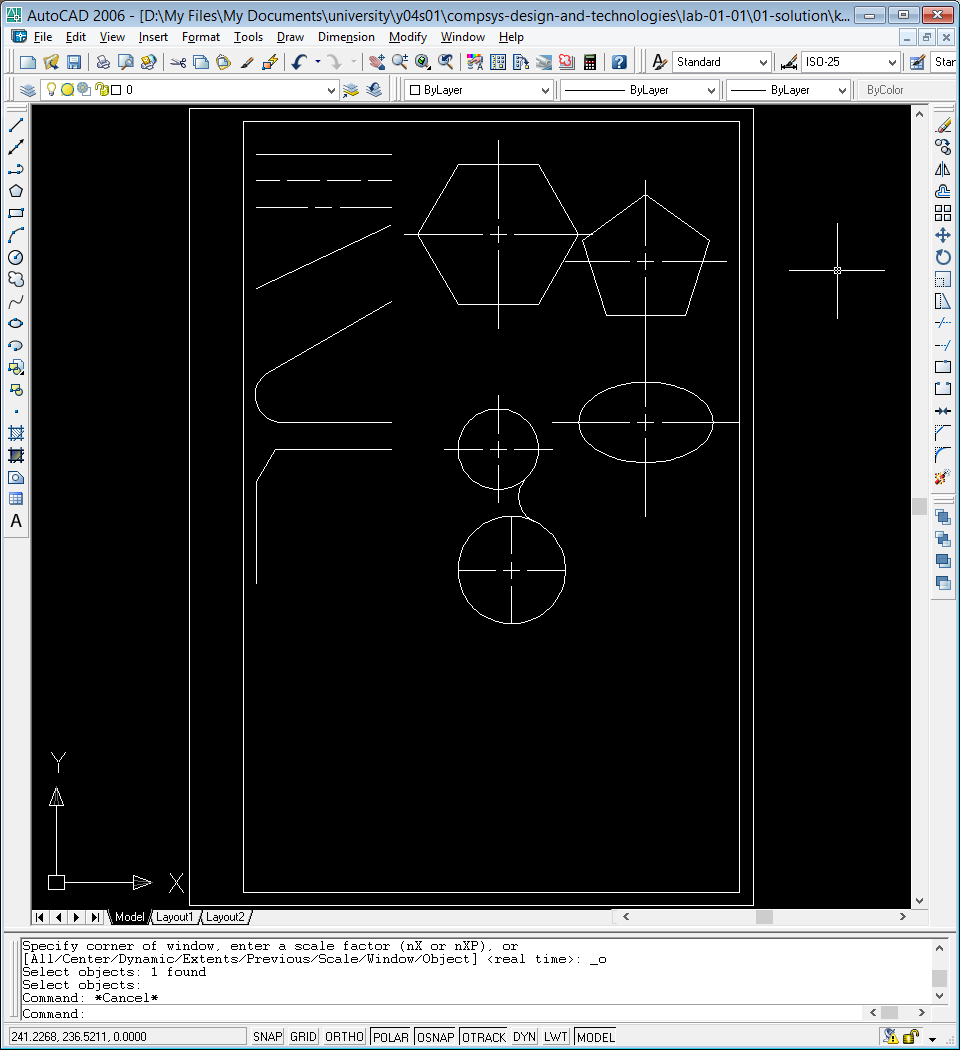
\includegraphics[height=19\baselineskip]{./assets/y04s01-csdt-lab-01-01-p10.png}
				\caption{Вигляд документа після побудови прямих, з'єднаних фаскою}
				\label{fig:08-chamfer-lines}
			\end{figure}

		\subsection{Побудова діаграми залежності~$y = f(x)$}
			Щоб~побудувати діаграму залежності, необхідно задати точки цієї залежності, які~визначені варіантом~(табл.~\ref{tab:points}). Перед початком побудови, встановимо стиль зображення точок, визначений завданням. Для~цього переходимо у~меню~\menu{Format > Point Style...} і~вибираємо необхідний стиль~(рис.~\ref{fig:09-point-style}).

			\begin{table}[!htbp]
				\centering
				\caption{Точки, задані за~варіантом}
				\label{tab:points}
				\begin{tabular}{
					v{2\gridunitwidth}
					n{2\gridunitwidth}
				}
					\toprule
						Номер точки & Координати\\
					\midrule
						1 & (20, 60) \\
						2 & (30, 49) \\
						3 & (40, 48) \\
						4 & (50, 43) \\
						5 & (60, 36) \\
						6 & (70, 20) \\
						7 & (80, 12) \\
					\bottomrule
				\end{tabular}
			\end{table}

			\begin{figure}[!htbp]
				\centering
				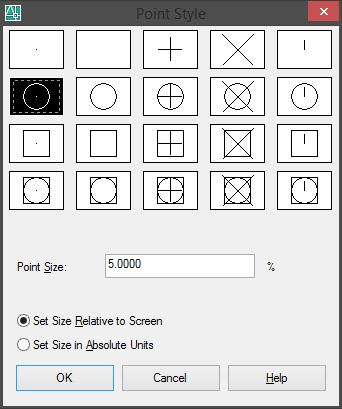
\includegraphics[height=12\baselineskip]{./assets/y04s01-csdt-lab-01-01-p11.png}
				\caption{Вікно вибору стилю точок}
				\label{fig:09-point-style}
			\end{figure}

			Встановивши необхідний стиль зображення точок, переходимо до~їх~побудови. Для~цього виконуємо такі команди:
			\begin{codegeneric}
				Command: point
				Current point modes:  PDMODE=0  PDSIZE=0.0000
				Specify a point: 20,60
				Command: point
				Current point modes:  PDMODE=0  PDSIZE=0.0000
				Specify a point: 30,49
				Command: point
				Current point modes:  PDMODE=0  PDSIZE=0.0000
				Specify a point: 40,48
				Command: point
				Current point modes:  PDMODE=0  PDSIZE=0.0000
				Specify a point: 50,43
				Command: point
				Current point modes:  PDMODE=0  PDSIZE=0.0000
				Specify a point: 60,36
				Command: point
				Current point modes:  PDMODE=0  PDSIZE=0.0000
				Specify a point: 70,20
				Command: point
				Current point modes:  PDMODE=0  PDSIZE=0.0000
				Specify a point: 80,12
			\end{codegeneric}
			Тепер у~документі з'явились точки необхідної діаграми. Щоб~побудувати власне діаграму, необхідно з'єднати ці~точки. З'єднання виконується за~допомогою сплайнів. Щоб~з'єднати точки за~допомогою сплайнів, виконаємо такі команди:
			\begin{codegeneric}
				Command: spline
				Specify first point or [Object]: 20,60
				Specify next point: 30,49
				Specify next point or [Close/Fit tolerance] <start tangent>: 40,48
				Specify next point or [Close/Fit tolerance] <start tangent>: 50,43
				Specify next point or [Close/Fit tolerance] <start tangent>: 60,36
				Specify next point or [Close/Fit tolerance] <start tangent>: 70,20
				Specify next point or [Close/Fit tolerance] <start tangent>: 80,12
				Specify next point or [Close/Fit tolerance] <start tangent>:
				Specify start tangent:
				Specify end tangent:
			\end{codegeneric}
			В~результаті отримали діаграму залежності~$y = f(x)$~(рис.~\ref{fig:10-function-diag}).

			\begin{figure}[!htbp]
				\centering
				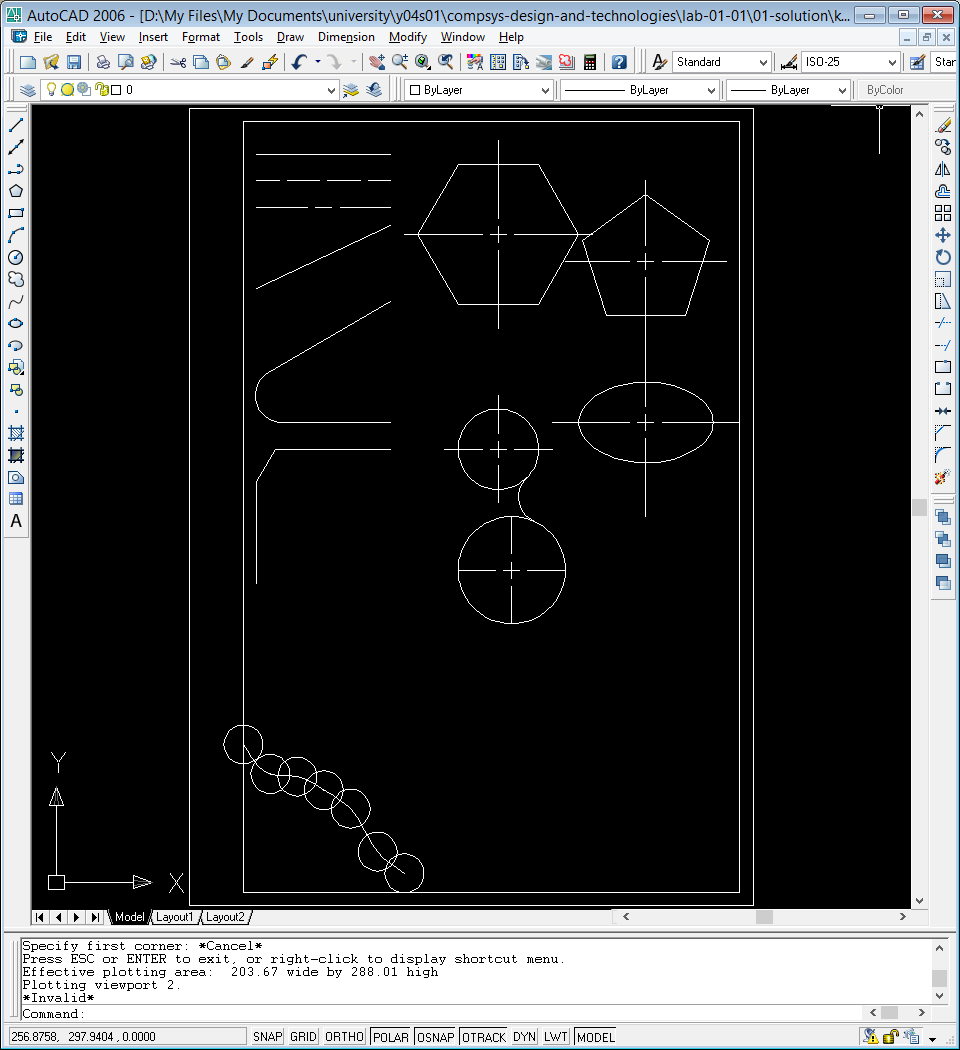
\includegraphics[height=18\baselineskip]{./assets/y04s01-csdt-lab-01-01-p12.png}
				\caption{Документ після побудови діаграми залежності~$y = f(x)$}
				\label{fig:10-function-diag}
			\end{figure}

	\section{Висновок}
		Виконуючи дану лабораторну роботу, ми~ознайомились з~пакетом проектування~\textenglish{Auto\allcaps{CAD}} і~оволоділи основними прийомами зображення простих графічних об'єктів в~ньому. Результатом виконання роботи став документ з побудованими фігурами.

		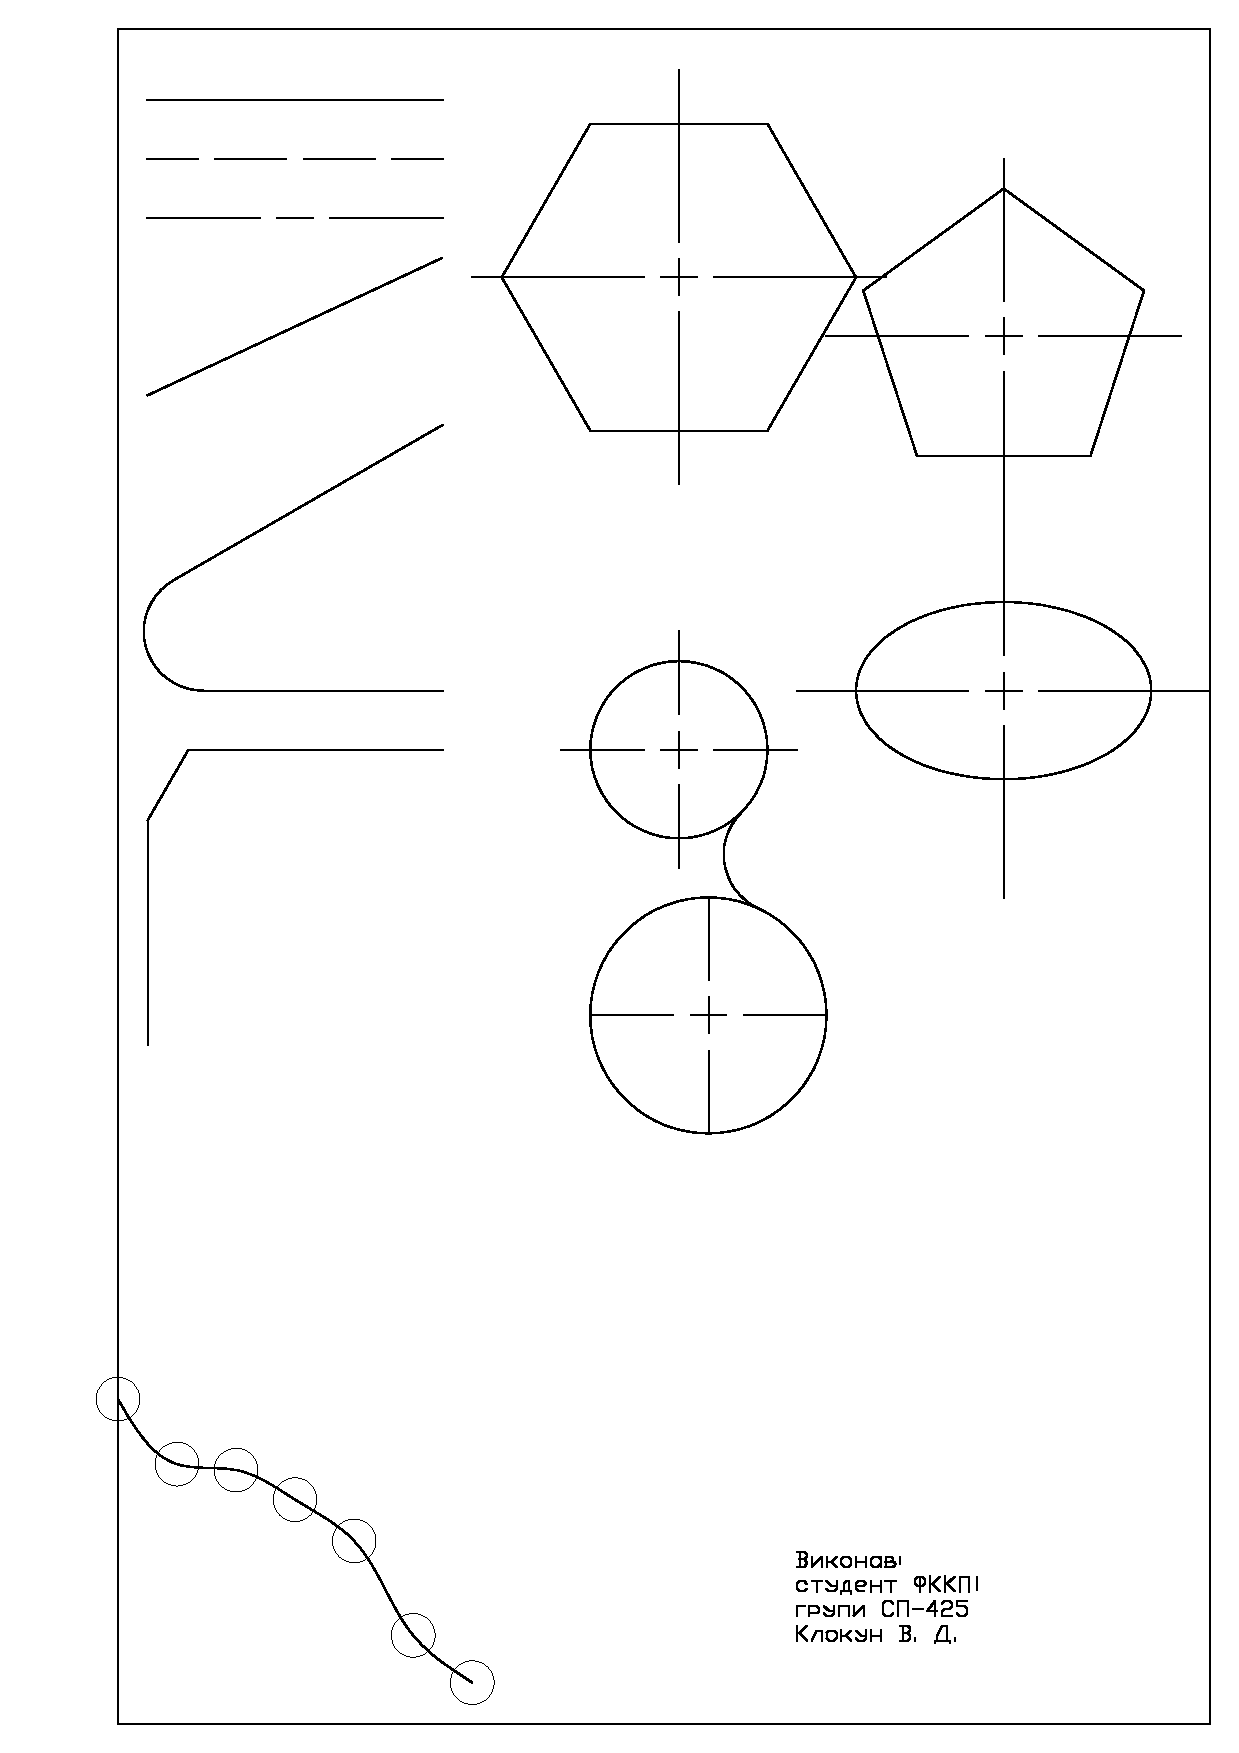
\includepdf[pages=-]{./assets/klokun-v05-var-08.pdf}

\end{document}
